\documentclass[a4paper,10pt]{article}
\usepackage[utf8x]{inputenc}

\usepackage{amsmath}
\usepackage{graphicx}

%opening
\title{Epipolar Geometry}
\author{Robrecht Jurriaans, Taco Cohen}

\begin{document}

\maketitle

\section{Estimating the Fundamental Matrix}
\label{sec:estF}
In order to estimate the 3D geometry of the scene from stereo images, we need to know the epipolar geometry of the setup.
The easiest treatment of epipolar geometry can be made when the image planes are parallel, but this is generally not the case for our input images.
For this reason, we first estimate the fundamental matrix $F$, that maps one image to another by a projective transformation.

To estimate $F$, we need correspondences, for which we will use points.
We find corresponding points in two images by matching Harris/Hessian Scale+Affine invariant descriptors.
Next, we center the two point-sets $\{p_i\}$ and $\{p'_i\}$ (one for each image), and scale the points so that the average distance to the mean is $\sqrt{2}$.
The matrices that perform this translation-scaling we call $T$ and $T'$.
As shown by Hartley \cite{Hartley}, this transformation improves the numerical stability of the following estimation procedure.
Our implementation of this procedure can be found in \verb+normalize.m+.

The Fundamental matrix is defined by the constraints
\begin{equation}
\mathbf{p_i'} F \mathbf{p_i} = 0
\end{equation}
which is linear in the parameters of $F$.
We form the matrix $A$ containing the coefficients of the linear equations in its rows, and solve $A \mathbf{f} = 0$ using SVD, where $\mathbf{f}$ is the matrix $F$ reshaped to a vector.

Finally, we enforce the `internal constraint' that $F$ must be singular (and that it must have exactly two non-zero singular values), by projecting it to the closest singular matrix, as measured by the projection F-norm.
It can be proved that this is achieved by simply zeroing the smallest singular value.
See \verb+singularizeF.m+ for our implementation.

\subsection{RANSAC}
Because the point correspondences will in general be noisy, the naive implementation described above will often yield poor results.
To get a more robust estimate, we apply the RANSAC algorithm.
RANSAC proceeds by iteratively estimating a transformation on a random sample of correspondences, determining inliers and re-estimating the transformation on the inliers.
Transformations resulting from good samples are retained, and after a number of iterations, the transformation with the highest inlier count is returned.
We make use of a theoretically sound termination criterion, as explained in our report for Assignment 3 of this course.

Our implementation of RANSAC for estimating the Fundamental matrix can be found in \verb+estimateFundamental.m+.
The code can be tested by running \verb+Fdemo.m+, whose output we discuss next.

\section{Results}

When \verb+Fdemo.m+ is run, three images are plotted.
The first, shown in figure \ref{fig:matches}, shows the matching points, and colored lines connecting putative matches.
Matches consistent with the RANSAC result (the inliers) are plotted in blue, while the outliers are drawn in red.

\begin{figure}[h!]
  \centering
    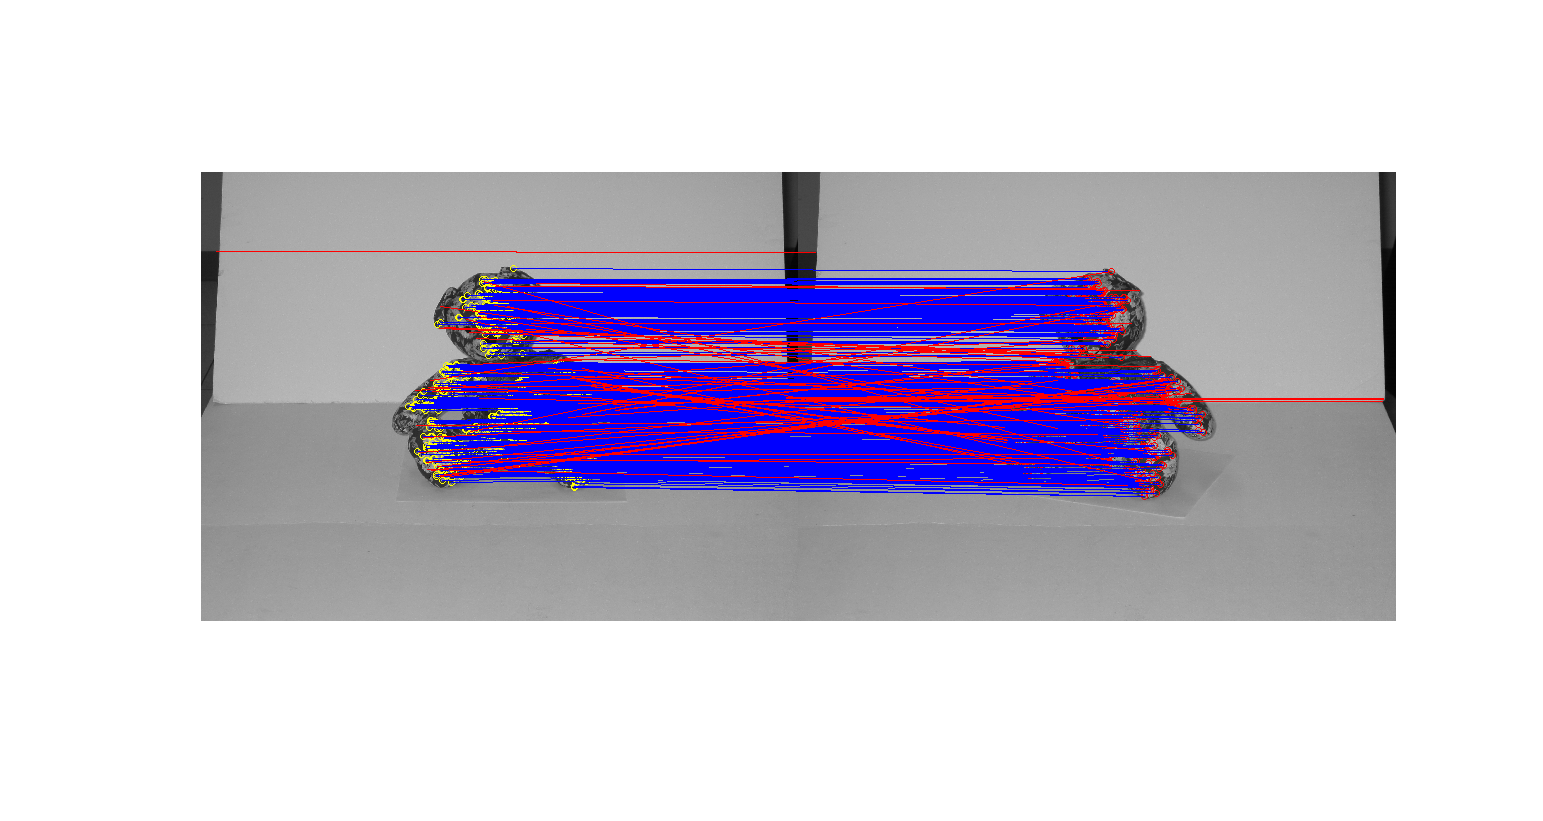
\includegraphics[width=1\textwidth]{TeddyMatch}
  \caption{Matches for the Teddy image. Blue are the inliers, red the outliers.}
  \label{fig:matches}
\end{figure}
 
The next output image, shown in figure \ref{fig:matches}, shows two randomly selected points, and the corresponding epipolar lines in the other image.
That is, the yellow point in the left image corresponds to the red line in the right image, and vice versa.
For a valid $F$, the epipolar line should pass through the point to which it corresponds in the other image, which is indeed the case in figure \ref{fig:matches}.
The lines are calculated using the standard formula for the epipolar line, $u_1 x + u_2 y + u_3 = 0$,
where $\mathbf{u} = F \mathbf{p}_l$ for the left point $\mathbf{p}_l$, and $\mathbf{u} = F^T \mathbf{p}_r$ for the right point.

\begin{figure}[h!]
  \centering
    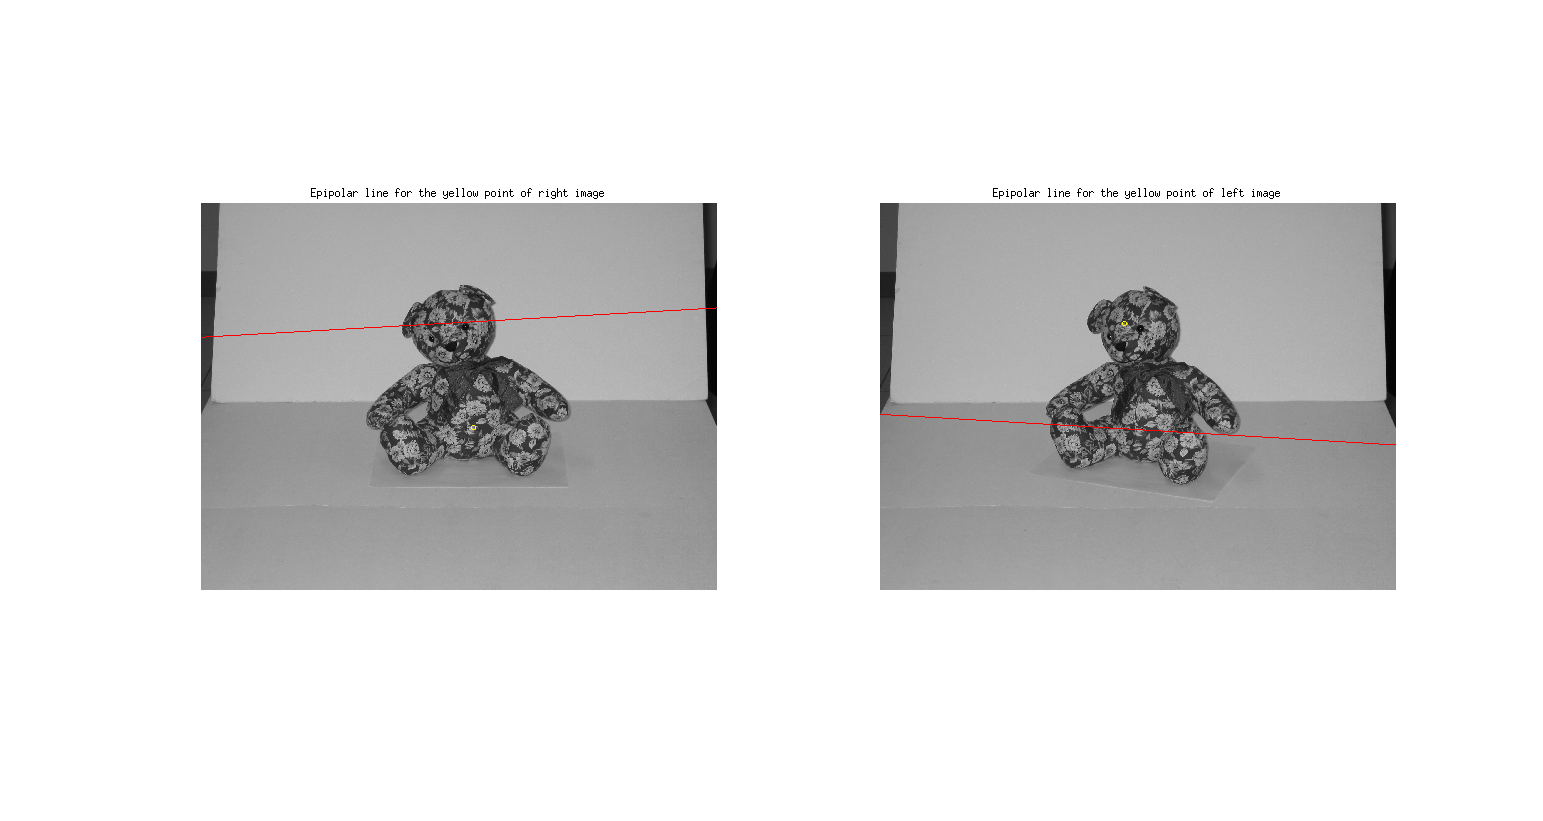
\includegraphics[width=1\textwidth]{EpipolarLines}
  \caption{Two randomly selected points (in yellow), and the corresponding epipolar line in the other image (red).}
  \label{fig:epilines}
\end{figure}


The third output image shows (at most) 20 matches, drawn as epipolar lines.
When the epipole is inside a view, it is plotted as a small circle.
The epipole, or rather its homogeneous representation, is simply the nullspace of $F$ or $F^T$, for the left and right image, respectively.
Although the correspondences between epipolar lines in both images are not plotted, it is clear that the lines are covariant with the camera transformation.

\begin{figure}[h!]
  \centering
    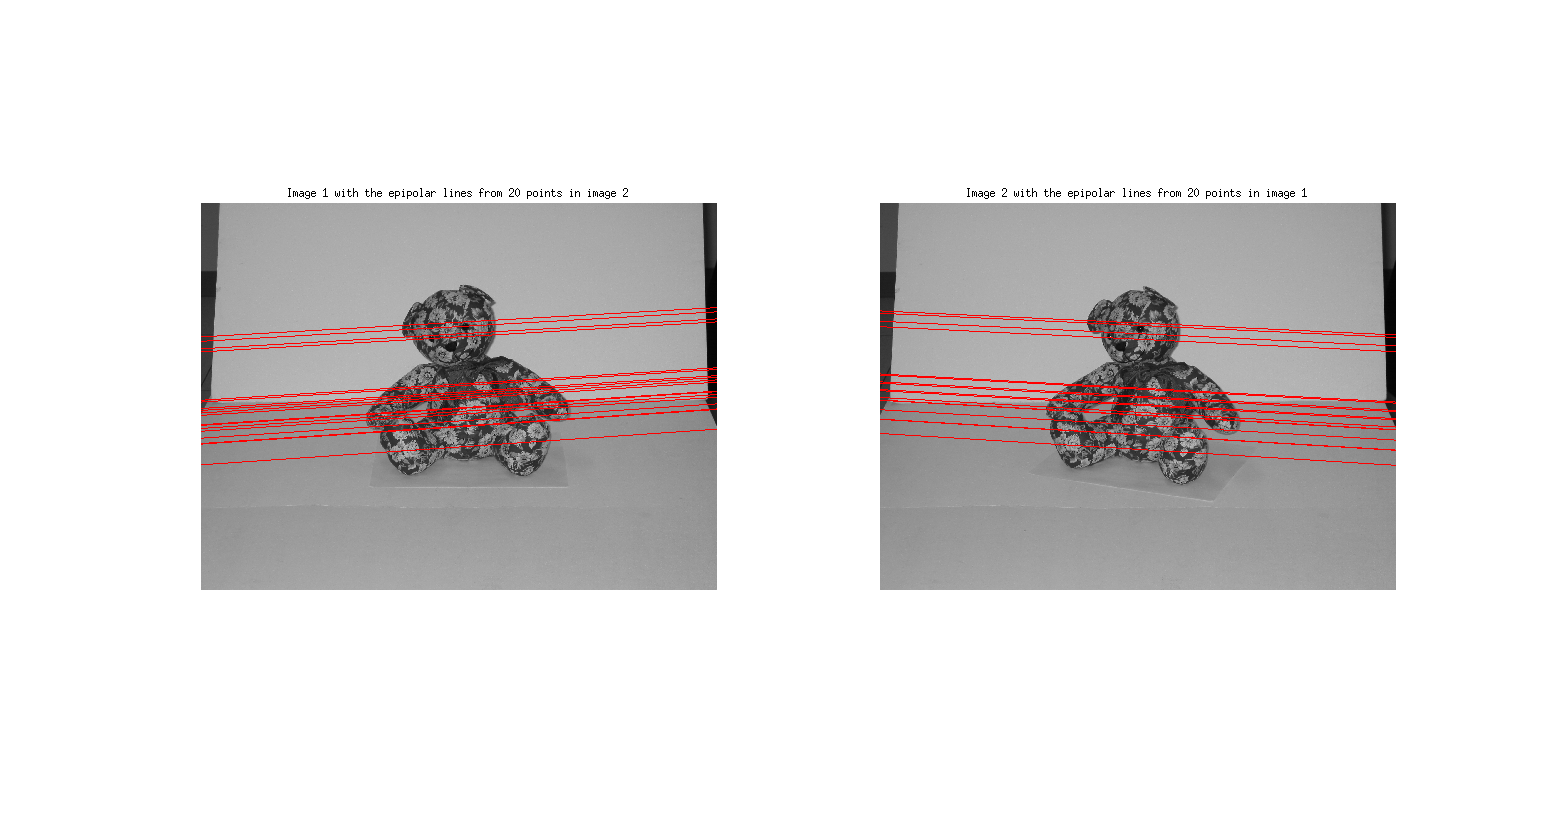
\includegraphics[width=1\textwidth]{Epipolarlines2}
  \caption{Epipolar lines representing corresponding keypoints in both images.}
  \label{fig:epi2}
\end{figure}



\subsection{The Fundamental Matrix}
When we estimate the Fundamental Matrix using the procedure described in section \ref{sec:estF}, we get a matrix such as
\begin{equation}
F = \begin{bmatrix}
-0.0000 & -0.0000 & 0.0006 \\
0.0000 & -0.0000 & -0.0119 \\
0.0003 & 0.0113 & -0.9999
\end{bmatrix}
\end{equation}
The extremely low values can be explained by two factors: the paralellism of the epipolar lines (see figure \ref{fig:epi2}), and the large scaling factor $d$ used in normalization.
Notice that the rows of $F$ each multiply the left point $\mathbf{p}_l$ to yield the parameters of the epipolar line, $u_1$, $u_2$ and $u_3$.
Since the lines are parallel, the slope, which is determined by $u_1$ and $u_2$, should be the same for each point.
This means that $u_1$ should not depend on the $x$ and $y$ coordinates of the point, so that the $F_{11}$ and $F_{12}$ must be (near) zero.
Similar reasoning explains the other two rows, and the near-symmetry of the matrix (since the analysis holds for $F^T \mathbf{p}_r$ too).



\bibliography{report}{}
\bibliographystyle{plain}


\end{document}
